\documentclass[a4paper]{amsart}

\usepackage{color}
\usepackage[colorlinks=true, citecolor=red]{hyperref}  %needs to come before amsrefs package to work with \cite{}*{}
\usepackage{amssymb,latexsym}
\usepackage[alphabetic]{amsrefs}
\usepackage[mathscr]{eucal}
\usepackage{pdfsync}
\usepackage{graphicx}
\usepackage{epstopdf}
\DeclareGraphicsRule{.tif}{png}{.png}{`convert #1 `dirname #1`/`basename #1 .tif`.png}
\usepackage[all]{xy}
\usepackage{titletoc}

\CompileMatrices

\theoremstyle{plain}
\newtheorem{theorem}{Theorem}[section]
\newtheorem{lemma}[theorem]{Lemma}
\newtheorem{proposition}[theorem]{Proposition}
\newtheorem{corollary}[theorem]{Corollary}

\theoremstyle{definition}
\newtheorem{definition}[theorem]{Definition}%[section]

\theoremstyle{remark}
\newtheorem{example}[theorem]{Example}
\newtheorem{remark}[theorem]{Remark}
\newtheorem{discussion}[theorem]{Discussion}
\DeclareMathOperator{\Lip}{Lip}
\DeclareMathOperator{\dist}{dist}
\DeclareMathOperator{\expected}{\mathbb{E}}
\DeclareMathOperator{\prb}{Prob}
\DeclareMathOperator{\spt}{spt}
\DeclareMathOperator{\lap}{\Delta}

\raggedbottom

\addtolength{\textwidth}{2cm}
\addtolength{\oddsidemargin}{-1cm}
\addtolength{\evensidemargin}{-1cm} 
\addtolength{\topmargin}{-1cm} 
\addtolength{\textheight}{2cm}
% \renewcommand{\l@subsection}{\@contentsline{2}{5em}{7em}}

%\makeatletter
%\makeatother

 
%%% BEGIN DOCUMENT
\begin{document}

\title{Models of an Economy}  
\author{John E.\ Hutchinson}
\date{\today}

\maketitle


%\renewcommand*\l@subsection{\@tocline{4}{50em}{7em}{10em}{10em}}


\tableofcontents







%%%%%%%%%%%%%%%%%%%%%%%%%%%%%%%%%%%%%
%%%%%%%%%%%%%%%%%%%%%%%%%%%%%%%%%%%%%%%%
%%%%%%%%%%%%%%%%%%%%%%%%%%%%%%%%%%%%%%%%%%
\section{\textbf{Introduction}}

We consider mathematical models of a trading economy with both a finite number of agents and a continuum of agents.  The latter:
\begin{enumerate}
\item is important as a limit model of the finite case;

\item is necessary in order to model an economy with a pricing system that cannot be influenced by individual agents;

\item is necessary if the notions of maximising individual preferences by commodity exchange, and maximising individual preferences by means of some pricing system, are to be equivalent.
\end{enumerate} 

Various generalisations are possible.  In particular, it is possible to include production.

\medskip The main references are \cites{HK, Hil1}.



%%%%%%%%%%%%%%%%%%%%%%%%%%%%%%%%%%%%%
%%%%%%%%%%%%%%%%%%%%%%%%%%%%%%%%%%%%%%%%
%%%%%%%%%%%%%%%%%%%%%%%%%%%%%%%%%%%%%%%%%%
\section{\textbf{Finite Exchange Economy}}


A \emph{finite}  \emph{exchange economy} $ \mathcal{E} = (\mathbb{R} ^\ell_+, \succeq_a, e_a; a \in A ) =  (\succeq_a, e_a; a \in A )$ is described by the \emph{primitive concepts} of   \emph{commodity space}, \emph{set of agents}, \emph{preference relation} and \emph{initial endowment}.

%%%%%%%%%%%%%%%%%%%%%%%
\subsection{Commodity Space}
A \emph{commodity} is a good or service.  It is represented by   points on $ \mathbb{R} _+ = [0,\infty) $. (And so commodities are ``infinitely divisible''.)

Assume there are $ \ell $ distinct commodities.

A \emph{commodity bundle} is a point in \emph{commodity space} $ \mathbb{R} ^\ell_+ := \{ (x_1,\dots, x_\ell) : x_i \geq 0 \ \forall i \} $.%
\footnote{For points $ x,y \in \mathbb{R} ^\ell $ we write   $ x \leq y $ if $ x_i \leq y_i \ \forall i $, and write $ x < y $ if $ x\leq y, x\neq y $.}

%%%%%%%%%%%%%%%%%%%%%%%%%%
\subsection{Set of Agents} There is a  \emph{finite} set $ A $ of \emph{agents} (\emph{traders}).


%%%%%%%%%%%%%%%%%%%%%%%%%%%%
\subsection{Preference Relations}
There is a  \emph{preference relation} (or desirability relation) $ \succeq_a $ for each $ a\in A $.  Thus is a binary relation on the \emph{consumption set} $ \mathbb{R} ^\ell_+ $.%
\footnote{It would be more realistic to restrict to a convex subset $ X $ of $ \mathbb{R} ^\ell_+ $, which may depend on $ a $ and represents the set of commodity bundles sufficient for the agent $ a $ to survive. The theory is essentially unchanged.}
 A generic preference relation is denoted by $ \succeq $.

$ x \succeq_a y $ is interpreted as ``for $ a $, $x $ is at least as desirable as $ y $''. i.e.\ ``$ x $ is as good as or better than~$ y $''.

\emph{Unless o.w.\  stated we assume}  $ \succeq $ is:
\begin{itemize} 

\item \emph{reflexive}: $ x \succeq x $;
\item \emph{complete}: $ x \succeq y $ or   $ y \succeq x $ (possibly both);
\item \emph{transitive}: $ x \succeq y   \text{ and } y \succeq z \Longrightarrow x \succeq z$;
\item \emph{continuous}:  $\{x : x \succeq y\} $ and  $\{x : y \succeq x\} $ are closed $\forall y \in \mathbb{R} ^\ell_+ $.
\end{itemize} 

Assuming just reflexivity and transitivity we define
\begin{enumerate}

\item $ x $ is \emph{as equally desirable as}   $ y $, written $ x \sim y $,  by $ x \succeq y $ and $ y \succeq x $  ($ x $ and $ y $ lie on the same indifference set for $ a $);
\item $ x $ is \emph{preferred to} (more desirable than) $ y $, written $ x \succ y $, by $ x \succeq y $ and not $ x \sim y $.
\end{enumerate}
Continuity is then equivalent to requiring that if $ x \succ  y $ then for all $ u $ in some nbd of $  x $ and all $ v $ in some nbd of $ y $, $ u \succ v $.


\medskip It  is often convenient to represent $ \succ $ by a \emph{Pareto utility function} $ u: \mathbb{R} ^\ell_+ \to \mathbb{R} $, where $ u(x) > u(y) $ iff $ x \succ y $.  Indifference sets are represented by   level sets  of $ u $.  See Figure~\ref{util}.


\begin{figure}[htbp] %  figure placement: here, top, bottom, or page
   \centering
   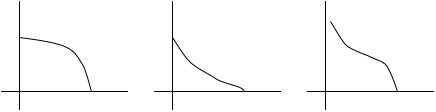
\includegraphics[width=3in]{util.jpg} 
   \caption{Possible level sets of $ \succ $.}
   \label{util}
\end{figure}

\medskip The following are further restrictions on the preference relations:

\emph{Monotonicity}: $y \geq x$  and $ y \neq x  \Longrightarrow y \succ x $.  (``more is better'')


 \emph{Convexity}: $ \{y: y \succeq x  \} $ to be  convex for all $ x \in \mathbb{R} ^\ell_+ $.

\emph{Strict convexity}: $ x \sim y,\ x \neq y,\  0<\lambda < 1 \Longrightarrow \lambda x + (1- \lambda ) y \succ y $. 
%%%%%%%%%%%%%%%%%%%%%%%%
\subsection{Initial Endowments} The \emph{initial endowment} (\emph{allocation}) for $ a $ is an element $ e_a \in \mathbb{R} ^\ell_+ \setminus \{0\} $. 

Every agent has non zero initial endowment as o.w.\ there  is nothing to trade and he will not be a part of the economy. 

 


%%%%%%%%%%%%%%%%%%%%%%%%%%%%%%%%%%%%%%%%%%%%%%%%%%
%%%%%%%%%%%%%%%%%%%%%%%%%%%%%%%%%%%%%%%%%%%%%%%%%%
%%%%%%%%%%%%%%%%%%%%%%%%%%%%%%%%%%%%%%%%%%%%%%%%%%
\section{\textbf{Redistribution in an Economy}}


\subsection{Defined concepts} 
Define the following for an economy $  \mathcal{E}   = (\succeq_a, e_a; a \in A )$:
\begin{enumerate}

\item A \emph{coalition} $ S $ is a \emph{non empty} subset of $ A $.

\item An \emph{allocation} is a map $ f:A \to \mathbb{R} ^\ell_+ $.  It is a \emph{redistribution} (\emph{feasible allocation}) if $ \sum_a f(a) = \sum_a e(a) $.  
(Conservation of commodities.)

\item A coalition $ S $ can \emph{improve upon} a redistribution $ f $ (using its \emph{original} endowment  $ \sum_{a\in S}   e(a)$)
if there is a redistribution $ g $ such that 
\begin{enumerate}

\item $ g(a) \succ f(a) $ for all $ a \in S $, (every agent in $ S $ has an improved situation)
\item $ \sum_{a\in S}  g(a) =  \sum_{a\in S}  e(a)$.   


\end{enumerate} 
W.l.o.g.\ one can take $ g(a) = f(a)\ \forall a \notin S $, i.e.\ only those resources in $ S $ are redistributed.
\end{enumerate} 

%%%%%%%%%%%%%%%%%%%%%%%%%%%%%%%%%%%%
\subsection{Edgeworth Box}

\begin{figure}[htbp] %  figure placement: here, top, bottom, or page
   \centering
   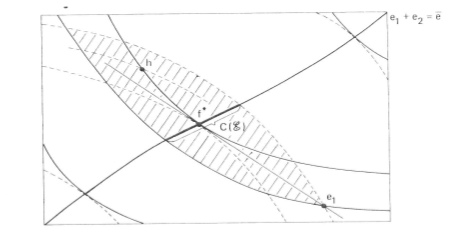
\includegraphics[width=4in]{edgeworth.jpg} 
   \caption{Two traders with two commodities.  See \cite{Hil2}*{p835}.}
   \label{edw}
\end{figure}

The ``Edgeworth Box'' in Figure~\ref{edw} represents two traders and two commodities.  One can do this in $ \mathbb{R} ^\ell $ for two traders and $ \ell $  commodities.

The origin for the first is in the lower left corner, the indifference lines  are solid, and the initial endowment is $ e_1$.  The origin for the second is in the upper right corner, the indifference lines  are dotted, and the initial endowment is $ e_2$.  
The total endowment is $ \overline{e} = e_1 + e_2 $ and so the initial endowment for \emph{both} traders  is represented by 
 the \emph{point} $ e_1 $ with origin   lower left corner --- this being the same as the  point $ e_2 $ with origin   upper right corner.   Each point in the box corresponds to a redistribution.

The coalition consisting of just the first trader can improve upon any allocation below the indifference line through $ e_1 $.   The coalition consisting of just the second trader can improve upon   any allocation above the dotted indifference line through $ e_1 $.  This leaves the shaded lens region. In here the coalition of both traders can improve upon any allocation which is not in the set of points $ \mathbb{C} (\mathcal{E} ) $ where indifference lines are tangential.



%%%%%%%%%%%%%%%%%%%%%%%%%%%%%%%%%%%%%%
\subsection{Core of an economy} The \emph{core} $ \mathbb{C} (\mathcal{E} ) $ of the economy $  \mathcal{E}   = (\succeq_a, e_a; a \in A )$ is the set  of all redistributions that no coalition can improve upon in the previous sense.%
\footnote{If such an allocation $ f $ is proposed, no coalition   will be able to improve on $ f $ by redistributing its \emph{original} endowment.   ***But could $ S $ improve the situation of all its members by redistributing the endowment obtained from $   f $ itself?***} 

\medskip
  That is, a redistribution $ f \in  \mathbb{C} (\mathcal{E} ) $ iff  no coalition can improve upon $ f $ by redistributing its \emph{initial} endowment.
More precisely, a redistribution $ f \in  \mathbb{C} (\mathcal{E} ) $ iff   there is   \emph{no} coalition $ S $ and redistribution  $ g $ 
such that
\begin{equation} \label{cnr}  
 \forall   a \in S\  \big(g(a) \succ f(a)\big)    \quad 
\text{and} \quad \sum_{a\in S}  g(a) =  \sum_{a\in S}  e(a).
\end{equation} 

%%%%%%%%%%%%%%%%%%%%%%%%%%%%%%%%%%%%%%%%%%
%%%%%%%%%%%%%%%%%%%%%%%%%%%%%%%%%%%%%%%%%%
%%%%%%%%%%%%%%%%%%%%%%%%%%%%%%%%%%%%%%%%%%
\section{\textbf{Prices in an Economy}}

Consider an economy $  \mathcal{E}   = (\succeq_a, e_a; a \in A )$.  We introduce an additional concept.


\subsection{Pricing System} A \emph{pricing system} or \emph{price vector} in $  \mathcal{E}   $ is a vector $ p \in \mathbb{R} ^\ell_+  $.  (Usually $ p>>0 $, i.e.\ $ p_i>0 \ \forall i$). The interpretation
is that $ p \cdot x = \sum_\ell p_\ell x_\ell $ is the price of the commodity bundle $ x \in  \mathbb{R} ^\ell_+$.
(We assume monotonicity.)

\medskip The \emph{budget set} for $ a\in A $, corresponding to the pricing system $ p $ and initial endowment  $e_a $, is 
\[ \beta(e_a, p) = \{ x \in \mathbb{R} ^\ell_+ : p \cdot x \leq p \cdot e_a \}. \]
It is interpreted as the set of commodity bundles that $ a $ can afford within his ``budget'' as given by $ p  $ and $ e_a $.

The \emph{income} of $ a $ is $ p \cdot a $.

 The \emph{demand set} for $ a\in A $ is
\begin{align*}
\phi(\succeq_a, e_a, p) &= \{   x \in\beta(e_a, p) : \not\exists y \in  \beta(e_a, p) \text{ s.t.\ } y \succ x \}\\
&=  \{   x \in\beta(e_a, p) :  y \in  \beta(e_a, p) \Longrightarrow x \succeq y \}\\
&= \{ x \in \mathbb{R} ^\ell_+ : p \cdot x  = p \cdot e_a\quad  \& \quad   y \succ x \Longrightarrow p\cdot y > p \cdot x \}.
\end{align*} 
It is the set of commodity bundles that $ a $ cannot improve upon within his budget, and is determined by his preferences, initial endowment and the pricing system.  In other words, it is the set of ``most preferred'' bundles available to $ a $ within his budget.

The demand set is a singleton  if the preference set is strictly convex and $ p >>0 $.
%%%%%%%%%%%%%%%%%%%%%%%%%%%%%%%%%%%%%%%%%%
\subsection{Walras Equilibrium}  A \emph{Walras equilibrium} for $ \mathcal{E}  $  is a redistribution $ f $ 
and a price system $ p $ such that, for every $ a \in A $, $ f(a) $   is in the demand set $ \phi(\succ_a, e_a, p)  $.   



More precisely,
\begin{equation} \label{}
\begin{gathered}
  f(a) \in \phi(\succ_a, e_a, p) \quad  \forall a \in A, \\
  \sum_{a\in A} f(a) =   \sum_{a\in A} e(a).
  \end{gathered} 
  \end{equation} 

In other words, $ (f,p) $ is a Walras equilibrium iff  no agent $ a $ can improve upon $ f(a) $  with the prevailing price system and his budget.
That is, 
\begin{equation} \label{weni}
   \forall a \in A\quad   x \succ_a f(a) \Longrightarrow p\cdot x > p\cdot f(a)  .
\end{equation} 


Alternatively,  a Wallas equilibrium is a redistribution  and a price system  such that \emph{total demand equals total supply}.  One also call this a \emph{price equilibrium}  or \emph{competitive equilibrium}.% 
\footnote{This is misleading terminology as there is not any competition involved.}  A Walras price system    \emph{decentralises the redistribution problem}.



\medskip
The redistribution $ f $ is called a \emph{Walras allocation} and the set of Walras allocations is denoted by $ \mathbb{W} (\mathcal{E} )$.

The price vector $ p $ is called a   \emph{Walras price vector} or \emph{equilibrium price vector}    and the set of equilibrium price vectors is denoted by $ \Pi(\mathcal{E} )$.  

 
\medskip In Figure~\ref{edw} the (unique) Walras equilibrium for the initial endowment $e_1 $  is $ (f^*,p) $, where $ p $ is normal to the line through $ e_1 $ and $ f^*$.

\medskip 

\begin{proposition}  $ \mathbb{W} (\mathcal{E} ) \subset   \mathbb{C} (\mathcal{E} )$. (\emph{No} assumptions on the structure of ``$ \succ $'' here.)
\end{proposition}

\begin{proof}  Assume $ f \in  \mathbb{W} (\mathcal{E} ) $ with equilibrium price vector $ p $.
Then by \eqref{weni} $ \forall a \in A $,
\begin{equation} \label{p1}
    x \succ_a f(a) \Longrightarrow p\cdot x > p\cdot f(a)  . 
\end{equation}

Assume $ f \notin  \mathbb{C} (\mathcal{E} )$.  Then by \eqref{cnr} $ \exists $ a redistribution $ g $ s.t.\ 
\begin{equation} \label{p2}
 \forall   a \in S\  \big(g(a) \succ_a f(a)\big)    \quad 
\text{and} \quad \sum_{a\in S}  g(a) =  \sum_{a\in S}  e(a).
\end{equation}

If $ a \in S $, one has from the first part of \eqref{p2}  that $ g(a) \succ_a f(a)$, and hence from \eqref{p1} that $ p\cdot g(a) > p\cdot e(a) $. Hence
$   p\cdot  \sum_{a\in S}  g(a) >  p\cdot \sum_{a\in S}  e(a) $. 

But from  the second part of \eqref{p2},  $   p\cdot  \sum_{a\in S}  g(a) =  p\cdot \sum_{a\in S}  e(a) $. 

This contradiction implies the second assumption is false and so $   \mathbb{W} (\mathcal{E} ) \subset   \mathbb{C} (\mathcal{E} )$.  
\end{proof} 





%%%%%%%%%%%%%%%%%%%%%%%%%%%%%%%%%%%%%%%%%%%%%%%
%%%%%%%%%%%%%%%%%%%%%%%%%%%%%%%%%%%%%%%%%%%%%%%%%%
%%%%%%%%%%%%%%%%%%%%%%%%%%%%%%%%%%%%%%%%%%%%%%%

\begin{thebibliography}{9} 

\bib{HK}{book}{
   author={Hildenbrand, W.},
   author={Kirman, A. P.},
   title={Equilibrium analysis},
   series={Advanced Textbooks in Economics},
   volume={28},
%   note={Variations on themes by Edgeworth and Walras},
   publisher={North-Holland Publishing Co.},
%   place={Amsterdam},
   date={1988},
   pages={xii+297},
%   isbn={0-444-70511-2},
%   review={\MR{1014892 (90m:90064)}},
}

\bib{Hil2}{article}{
   author={Hildenbrand, Werner},
   title={Core of an Economy},
   book={
      editor={Arrow, K.J},
      editor={Intriligator, M.D},
      title={Handbook of Mathematical Economics},
      publisher={North-Holland},
       chapter={18},
   },
         date={1982},
   pages={831--877},
}


\bib{Hil1}{book}{
   author={Hildenbrand, Werner},
   title={Core and equilibria of a large economy},
  note={
   Princeton Studies in Mathematical Economics, No. 5},
   publisher={Princeton University Press},
%   place={Princeton, N.J.},
   date={1974},
   pages={viii+251},
%   review={\MR{0389160 (52 \#9991)}},
}



\end{thebibliography}

\end{document}





\end{thebibliography}





\end{document}


